\documentclass{zirkelblatt}

\usepackage{geometry,wrapfig}
\geometry{tmargin=0.5cm,bmargin=0.5cm,lmargin=1cm,rmargin=1cm}

\pagestyle{empty}

\makeatletter
\newcommand*{\shifttext}[2]{%
  \settowidth{\@tempdima}{#2}%
  \makebox[\@tempdima]{\hspace*{#1}#2}%
}
\makeatother

\begin{document}

\selectlanguage{english}

\newcommand{\vorderseite}{
  \begin{minipage}[t][4cm][t]{7.6cm}
    \begin{center}
      \textsf{Graham's number} \\
      \tiny
      \textsf{an enormous number in Ramsey theory}
      \vspace{0.6em}

      \makebox[0pt]{\shifttext{-10pt}{\ldots}}%
      \scalebox{1.00}{024 259 5069 506 473 8395 657 479 1365 193 517 9833 453 536 2521}

      \scalebox{1.00}{430 035 4012 602 677 1622 672 160 4198 106 522 6316 935 518 8780}

      \scalebox{1.00}{388 144 8314 065 252 6168 785 095 5526 460 510 7117 200 099 7092}			

      \scalebox{1.00}{912 495 4437 888 749 6062 882 911 7250 630 013 0362 293 491 6080}			

      \scalebox{1.00}{254 594 6149 457 887 1427 832 350 8292 421 020 9182 589 675 3560}			

      \scalebox{1.00}{430 869 9380 168 924 9889 268 099 5101 690 559 1995 119 502 7887}			

      \scalebox{1.00}{178 308 3701 834 023 6474 548 882 2221 615 732 2801 013 297 4509}			

      \scalebox{1.00}{273 445 9450 434 330 0901 096 928 0253 527 518 3328 988 446 1508}			

      \scalebox{1.00}{940 424 8265 018 193 8515 625 357 9639 961 899 3967 905 496 6380}			

      \scalebox{1.00}{032 223 4872 396 701 8485 186 439 0591 045 756 2726 246 419 5387}			
    \end{center}
  \end{minipage}
}

\newcommand{\rueckseite}{
  \begin{minipage}[t][4cm][t]{7.6cm}
    \phantom{A}
    \vspace{-0.3em}
    \tiny

    %\begin{wrapfigure}{l}{0.5cm}
    %  \vspace*{-0.4cm}
    %  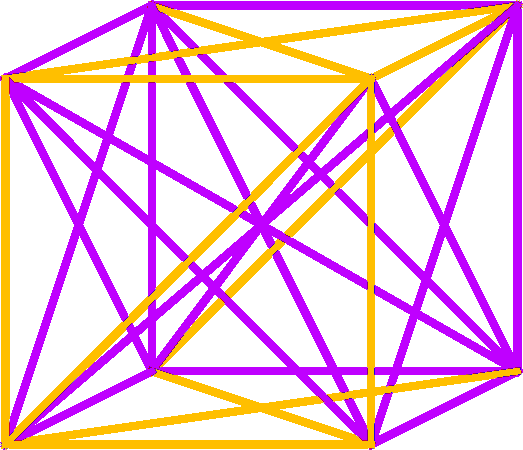
\includegraphics[trim,scale=0.30]{monophilic-coloring}
    %  \vspace*{-0.6cm}
    %\end{wrapfigure}
    This coloring of the edges connecting any two vertices
    of the cube is \textbf{monophilic} because it
    contains a singly-colored plane region spanned by four vertices.
    But not all colorings of the cube are monophilic,
    and similarly for the four-, five-, \ldots, and 13-dimensional cube.
    In contrast, any coloring of the $G$-dimensional cube is monophilic.
    The definition of~$G$ uses \textbf{hyperoperators}:
    \begin{multicols*}{2}
    \quad\qquad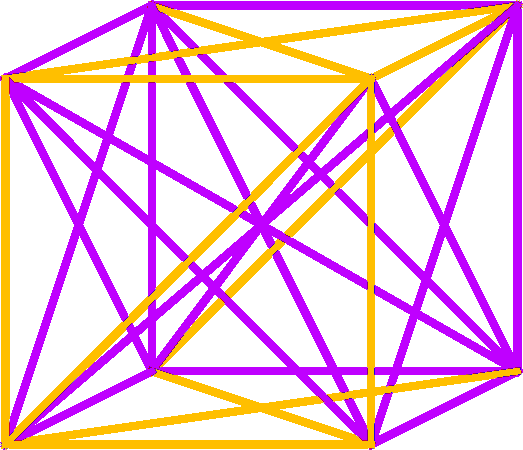
\includegraphics[scale=0.30]{monophilic-coloring}
    \vspace*{-1em}
    \begin{align*}
      2 \uparrow\uparrow 4 &= 2^{2^{2^2}} = 65536 \\
      2 \uparrow\uparrow\uparrow 4 &= 2 \uparrow\uparrow (2 \uparrow\uparrow (2
      \uparrow\uparrow 2))
    \end{align*}
    \columnbreak
    $\left.\!\!\!\!\!\!\!\!\!\!\!\!\!\!\!\!\!\!\!\!\!\!\!
       \begin{matrix}
	G\!\!\!\!\! &=\!\!\!\!\!&3\underbrace{\uparrow \cdots \cdots \cdots \cdots \cdots \uparrow}3 \\
	  & &3\underbrace{\uparrow \cdots \cdots \cdots \cdots \uparrow}3 \\[-0.4em]
	  & & \underbrace{\qquad \quad \vdots \qquad \quad} \\
	  & &3\underbrace{\uparrow \cdots \cdots \uparrow}3 \\
	  & &3\uparrow \uparrow \uparrow \uparrow3
       \end{matrix}
      \right \} \text{64 layers}
      $
    \end{multicols*}
  \end{minipage}
}

\vorderseite\hfill\vorderseite
\vfill
\vorderseite\hfill\vorderseite
\vfill
\vorderseite\hfill\vorderseite
\vfill
\vorderseite\hfill\vorderseite
\vfill
\vorderseite\hfill\vorderseite

\newpage

%\fontfamily{kurier}\selectfont

\rueckseite\hfill\rueckseite
\vfill
\rueckseite\hfill\rueckseite
\vfill
\rueckseite\hfill\rueckseite
\vfill
\rueckseite\hfill\rueckseite
\vfill
\rueckseite\hfill\rueckseite

\end{document}


\newcommand{\vorderseite}{
  \begin{minipage}[t][4cm][t]{7.6cm}
    \begin{center}
        \textsf{Grahams Zahl}
        \vspace{0.6em}
        \end{center}
          \tiny
          Grahams Zahl $G_{64}$ ist eine ganz spezielle natürliche Zahl $\mathbb{N}$, sie ist sehr groß, so extrem groß, dass nicht einmal der Hyperpotenz-Operator (diesen nutzt man wenn normales potenzieren nicht mehr aussreicht) ausreicht, um diese Zahl direkt anzugeben.
          Trotz ihrer nahezu unvorstellbaren Größe kann man die letzten Stellen von Grahams Zahl mit elementarer Zahlentheorie bestimmen. Die letzten 500 Stellen von Grahams Zahl lauten:	
          \end{minipage}
}

\newcommand{\rueckseite}{
	\begin{minipage}[t][4cm][t]{7.6cm}
		\phantom{A}
		\vspace{-0.3em}
		\tiny
		\begin{center}
	
			\scalebox{1.00}{024 259 5069 506 473 8395 657 479 1365 193 517 9833 453 536 2521}
			
			\scalebox{1.00}{430 035 4012 602 677 1622 672 160 4198 106 522 6316 935 518 8780}
			
			\scalebox{1.00}{388 144 8314 065 252 6168 785 095 5526 460 510 7117 200 099 7092}			
			
			\scalebox{1.00}{912 495 4437 888 749 6062 882 911 7250 630 013 0362 293 491 6080}			
			
			\scalebox{1.00}{254 594 6149 457 887 1427 832 350 8292 421 020 9182 589 675 3560}			
			
			\scalebox{1.00}{430 869 9380 168 924 9889 268 099 5101 690 559 1995 119 502 7887}			
			
			\scalebox{1.00}{178 308 3701 834 023 6474 548 882 2221 615 732 2801 013 297 4509}			
			
			\scalebox{1.00}{273 445 9450 434 330 0901 096 928 0253 527 518 3328 988 446 1508}			
			
			\scalebox{1.00}{940 424 8265 018 193 8515 625 357 9639 961 899 3967 905 496 6380}			
			
			\scalebox{1.00}{032 223 4872 396 701 8485 186 439 0591 045 756 2726 246 419 5387}			
			
		\end{center}
		
	\end{minipage}
}

	\vorderseite\hfill\vorderseite
	\vfill
	\vorderseite\hfill\vorderseite
	\vfill
	\vorderseite\hfill\vorderseite
	\vfill
	\vorderseite\hfill\vorderseite
	\vfill
	\vorderseite\hfill\vorderseite
	
	\newpage
	
	\fontfamily{kurier}\selectfont
	
	\rueckseite\hfill\rueckseite
	\vfill
	\rueckseite\hfill\rueckseite
	\vfill
	\rueckseite\hfill\rueckseite
	\vfill
	\rueckseite\hfill\rueckseite
	\vfill
	\rueckseite\hfill\rueckseite
		
\end{document}

